\documentclass[12pt,a4paper,BCOR12mm, headexclude, footexclude, twoside, openright]{scrartcl} 
\usepackage[scaled]{helvet}
\usepackage[british]{babel}
\usepackage[utf8]{inputenc}
\usepackage[T1]{fontenc}
\usepackage{fancyhdr}
\usepackage{lastpage}
\usepackage{ifthen}
\usepackage{amsmath,amsfonts,amsthm}
\usepackage{sfmath}
\usepackage{makecell}
\usepackage{booktabs}
\usepackage{sectsty}
\usepackage{xcolor}
\usepackage{tikz}
%\KOMAoptions{optionenliste}
%\KOMAoptions{Option}{Werteliste}

\newcommand*{\TakeFourierOrnament}[1]{{%
\fontencoding{U}\fontfamily{futs}\selectfont\char#1}}
\newcommand*{\danger}{\TakeFourierOrnament{66}}
\addtokomafont{caption}{\small}
%\setkomafont{descriptionlabel}{\normalfont
%	\bfseries}
\setkomafont{captionlabel}{\normalfont
	\bfseries}
\let\oldtabular\tabular
\renewcommand{\tabular}{\sffamily\oldtabular}
\KOMAoptions{abstract=true}
%\setkomafont{footnote}{\sffamily}
%\KOMAoptions{twoside=true}
%\KOMAoptions{headsepline=true}
%\KOMAoptions{footsepline=true}
\renewcommand\familydefault{\sfdefault}
\renewcommand{\arraystretch}{1.1}
\newcommand{\horrule}[1]{\rule{\linewidth}{#1}}
\setlength{\textheight}{230mm}
\allsectionsfont{\centering \normalfont\scshape}
\let\tmp\oddsidemargin
\let\oddsidemargin\evensidemargin
\let\evensidemargin\tmp
\reversemarginpar

\numberwithin{equation}{section} % Number equations within sections (i.e. 1.1, 1.2, 2.1, 2.2 instead of 1, 2, 3, 4)
\numberwithin{figure}{section} % Number figures within sections (i.e. 1.1, 1.2, 2.1, 2.2 instead of 1, 2, 3, 4)
\numberwithin{table}{section} % Number tables within sections (i.e. 1.1, 1.2, 2.1, 2.2 instead of 1, 2, 3, 4)

\setlength\parindent{0pt}

\definecolor{C000000}{HTML}{000000}
\definecolor{CFFFFFF}{HTML}{FFFFFF}
\definecolor{C00FF00}{HTML}{00FF00}
\begin{document}
%\sffamily
\fancypagestyle{plain}
{%
  \renewcommand{\headrulewidth}{0pt}%
  \renewcommand{\footrulewidth}{0.5pt}
  \fancyhf{}%
  \fancyfoot[R]{\emph{\footnotesize Page \thepage\ of \pageref{LastPage}}}%
  \fancyfoot[C]{\emph{\footnotesize Samy Aittahar}}%
}

\thispagestyle{plain}

\titlehead
{
	University of Liège\hfill
    INFO8006%
}

\subject{\vspace{-1.0ex} \horrule{2pt}\\[0.15cm] {\textsc{\texttt{Introduction to AI}}}}
\title{Project : $N \times M \times K$ Tic Tac Toe \\}
\subtitle{\textsc{\texttt{Not 3D}}\\\horrule{2pt}\\[0.5cm]}
\author{\bfseries{Samy Aittahar}\vspace{-2ex}}
\date{\begin{tabular}{cc}
  \textsc{Date:}& \textsc{\emph{\today}}
\end{tabular}}
\maketitle

%\begin{abstract}
%\end{abstract}

%--------------------------------------------

\section{Pratical Informations}
\begin{itemize}
	\item Individual project ;
    \item Deadline : TBA, should be end of November ? ;
    \item Deliverable : A python file with a class named "Solver" which can be initialised with \emph{Solver(X)} which has to implement the following function : $solve(M)$, where $M$ is a NumPy matrix of integers and $X$ your symbol (either 1 or 2), which return a tuple (A,B) with A and B strictly positive natural numbers ;
    \begin{itemize}
    	\item \danger If your tuple violates the game constraints, you simply miss the turn ;
    \end{itemize}
    \item Send your deliverable to saittahar@ulg.ac.be with the subject \emph{name}\_tictactoe, and with enclosed a file with the same name and \emph{.py} extension

\end{itemize}
\newpage
\section{$N \times M$ Tic Tac Toe Grid}
\begin{center}
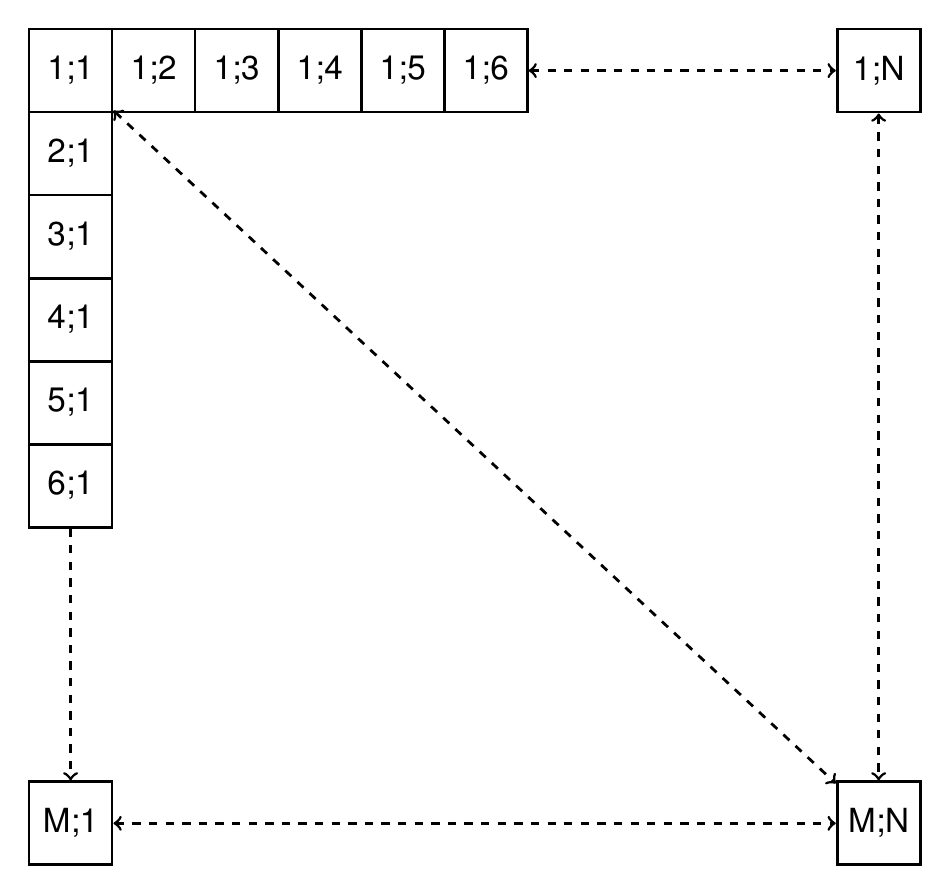
\begin{tikzpicture}[inner sep=0pt]
\node (n0) [minimum height=30.0pt, minimum width=30.0pt,at={(377pt,-230pt)}, fill=white, draw, line width=1.0pt,align=center,text width=23.3125,font=\fontfamily{phv}\fontsize{12}{13}\selectfont, shape=rectangle] {1;1};
\node (n1) [minimum height=30.0pt, minimum width=30.0pt,at={(407pt,-230pt)}, fill=white, draw, line width=1.0pt,align=center,text width=23.3125,font=\fontfamily{phv}\fontsize{12}{13}\selectfont, shape=rectangle] {1;2};
\node (n2) [minimum height=30.0pt, minimum width=30.0pt,at={(437pt,-230pt)}, fill=white, draw, line width=1.0pt,align=center,text width=23.3125,font=\fontfamily{phv}\fontsize{12}{13}\selectfont, shape=rectangle] {1;3};
\node (n3) [minimum height=30.0pt, minimum width=30.0pt,at={(497pt,-230pt)}, fill=white, draw, line width=1.0pt,align=center,text width=23.3125,font=\fontfamily{phv}\fontsize{12}{13}\selectfont, shape=rectangle] {1;5};
\node (n4) [minimum height=30.0pt, minimum width=30.0pt,at={(527pt,-230pt)}, fill=white, draw, line width=1.0pt,align=center,text width=23.3125,font=\fontfamily{phv}\fontsize{12}{13}\selectfont, shape=rectangle] {1;6};
\node (n5) [minimum height=30.0pt, minimum width=30.0pt,at={(669pt,-230pt)}, fill=white, draw, line width=1.0pt,align=center,text width=24.654296875,font=\fontfamily{phv}\fontsize{12}{13}\selectfont, shape=rectangle] {1;N};
\node (n6) [minimum height=30.0pt, minimum width=30.0pt,at={(467pt,-230pt)}, fill=white, draw, line width=1.0pt,align=center,text width=23.3125,font=\fontfamily{phv}\fontsize{12}{13}\selectfont, shape=rectangle] {1;4};
\node (n7) [minimum height=30.0pt, minimum width=30.0pt,at={(377pt,-260pt)}, fill=white, draw, line width=1.0pt,align=center,text width=23.3125,font=\fontfamily{phv}\fontsize{12}{13}\selectfont, shape=rectangle] {2;1};
\node (n8) [minimum height=30.0pt, minimum width=30.0pt,at={(377pt,-290pt)}, fill=white, draw, line width=1.0pt,align=center,text width=23.3125,font=\fontfamily{phv}\fontsize{12}{13}\selectfont, shape=rectangle] {3;1};
\node (n9) [minimum height=30.0pt, minimum width=30.0pt,at={(377pt,-320pt)}, fill=white, draw, line width=1.0pt,align=center,text width=23.3125,font=\fontfamily{phv}\fontsize{12}{13}\selectfont, shape=rectangle] {4;1};
\node (n10) [minimum height=30.0pt, minimum width=30.0pt,at={(377pt,-350pt)}, fill=white, draw, line width=1.0pt,align=center,text width=23.3125,font=\fontfamily{phv}\fontsize{12}{13}\selectfont, shape=rectangle] {5;1};
\node (n11) [minimum height=30.0pt, minimum width=30.0pt,at={(377pt,-380pt)}, fill=white, draw, line width=1.0pt,align=center,text width=23.3125,font=\fontfamily{phv}\fontsize{12}{13}\selectfont, shape=rectangle] {6;1};
\node (n12) [minimum height=30.0pt, minimum width=30.0pt,at={(377pt,-502pt)}, fill=white, draw, line width=1.0pt,align=center,text width=26.03125,font=\fontfamily{phv}\fontsize{12}{13}\selectfont, shape=rectangle] {M;1};
\node (n13) [minimum height=30.0pt, minimum width=30.0pt,at={(669pt,-502pt)}, fill=white, draw, line width=1.0pt,align=center,text width=27.373046875,font=\fontfamily{phv}\fontsize{12}{13}\selectfont, shape=rectangle] {M;N};


\path [to-to,line width=1.0pt,draw,dashed,](n4)--(n5);


\path [-to,line width=1.0pt,draw,dashed,](n11)--(n12);


\path [to-to,line width=1.0pt,draw,dashed,](n0)--(n13);


\path [to-to,line width=1.0pt,draw,dashed,](n12)--(n13);


\path [to-to,line width=1.0pt,draw,dashed,](n5)--(n13);
\end{tikzpicture}
\end{center}

This is a classical tic tac toe grid. You'll notice that the grid can be really large. Plus, it is not necessarily a square.

Usually, we denote 'X' and 'O' for each player token, but in this project we'll go for $1$ and $2$ ($0$ is empty).\\

The rules\footnote{For a quick reminder : https://en.wikipedia.org/wiki/Tic-tac-toe} remain the same, except the following. Instead to have most complete diagonals/lines/columns with the same symbol, players are expected to cumulate subdiagonals/sublines/subcolumns of size $K$ (denoted as $K$-alignment) with the same symbol.\\
For each of them, the player earns 1 point. Plus, if a symbol is at an intersection of $i$ $K-1$ alignments, those are counted as $i$ distincts $K$ alignments. When a symbol is used at an intersection, this rule does not apply to symbols along the same direction for which the distance from this former is less than $K-1$. Finally, when a player build at least 1 $K$-alignment, he also takes the next turn.\\ 

Thus, the goal is to have more points than the opponent at the point where it is not possible for any of the players to build more $K$-alignments. The game is made more challenging with a budget time limit of 1 minute.\\

You'll find below some common scoring examples with a $10 \times 10$ grid and $K = 5$.

\begin{figure}
\begin{center}
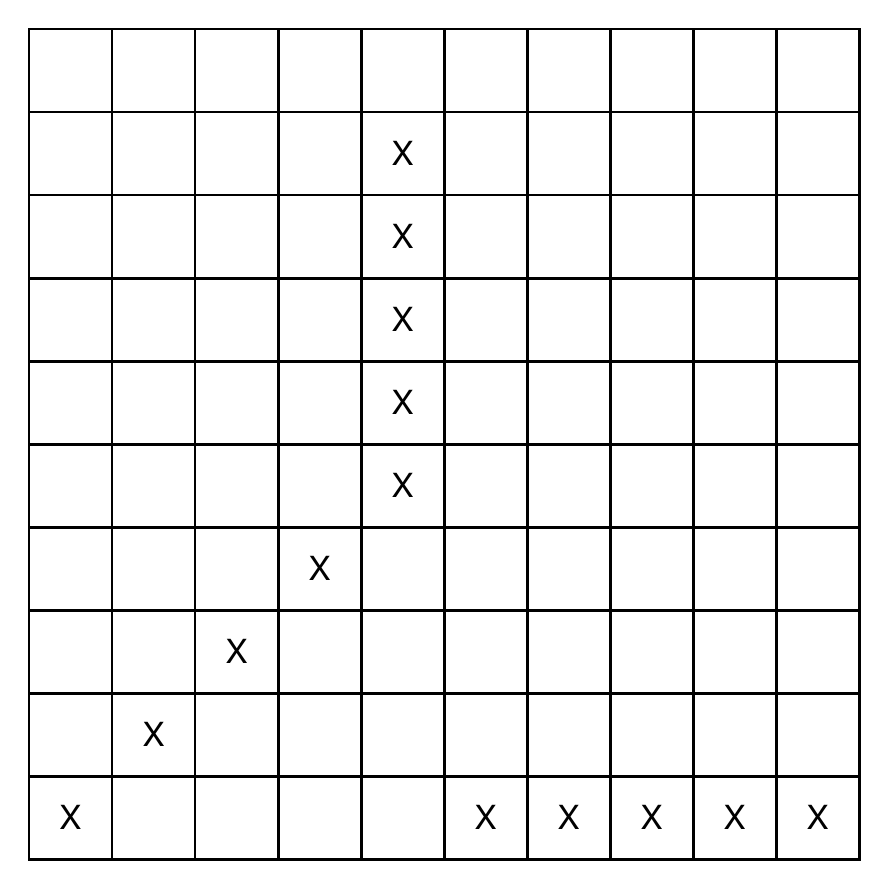
\begin{tikzpicture}[inner sep=0pt,scale=1]
\node (n0) [minimum height=30.0pt, minimum width=30.0pt,at={(270pt,-150pt)}, fill=white, draw, line width=1.0pt,align=center,text width=11.634765625,font=\fontfamily{phv}\fontsize{12}{13}\selectfont, shape=rectangle] {};
\node (n1) [minimum height=30.0pt, minimum width=30.0pt,at={(300pt,-150pt)}, fill=white, draw, line width=1.0pt,align=center,text width=11.634765625,font=\fontfamily{phv}\fontsize{12}{13}\selectfont, shape=rectangle] {};
\node (n2) [minimum height=30.0pt, minimum width=30.0pt,at={(330pt,-150pt)}, fill=white, draw, line width=1.0pt,align=center,text width=11.634765625,font=\fontfamily{phv}\fontsize{12}{13}\selectfont, shape=rectangle] {};
\node (n3) [minimum height=30.0pt, minimum width=30.0pt,at={(360pt,-150pt)}, fill=white, draw, line width=1.0pt,align=center,text width=11.634765625,font=\fontfamily{phv}\fontsize{12}{13}\selectfont, shape=rectangle] {};
\node (n4) [minimum height=30.0pt, minimum width=30.0pt,at={(390pt,-150pt)}, fill=white, draw, line width=1.0pt,align=center,text width=11.634765625,font=\fontfamily{phv}\fontsize{12}{13}\selectfont, shape=rectangle] {};
\node (n5) [minimum height=30.0pt, minimum width=30.0pt,at={(420pt,-150pt)}, fill=white, draw, line width=1.0pt,align=center,text width=11.634765625,font=\fontfamily{phv}\fontsize{12}{13}\selectfont, shape=rectangle] {};
\node (n6) [minimum height=30.0pt, minimum width=30.0pt,at={(450pt,-150pt)}, fill=white, draw, line width=1.0pt,align=center,text width=11.634765625,font=\fontfamily{phv}\fontsize{12}{13}\selectfont, shape=rectangle] {};
\node (n7) [minimum height=30.0pt, minimum width=30.0pt,at={(480pt,-150pt)}, fill=white, draw, line width=1.0pt,align=center,text width=11.634765625,font=\fontfamily{phv}\fontsize{12}{13}\selectfont, shape=rectangle] {};
\node (n8) [minimum height=30.0pt, minimum width=30.0pt,at={(510pt,-150pt)}, fill=white, draw, line width=1.0pt,align=center,text width=11.634765625,font=\fontfamily{phv}\fontsize{12}{13}\selectfont, shape=rectangle] {};
\node (n9) [minimum height=30.0pt, minimum width=30.0pt,at={(540pt,-150pt)}, fill=white, draw, line width=1.0pt,align=center,text width=19.26953125,font=\fontfamily{phv}\fontsize{12}{13}\selectfont, shape=rectangle] {};
\node (n10) [minimum height=30.0pt, minimum width=30.0pt,at={(270pt,-180pt)}, fill=white, draw, line width=1.0pt,align=center,text width=19.26953125,font=\fontfamily{phv}\fontsize{12}{13}\selectfont, shape=rectangle] {};
\node (n11) [minimum height=30.0pt, minimum width=30.0pt,at={(300pt,-180pt)}, fill=white, draw, line width=1.0pt,align=center,text width=19.26953125,font=\fontfamily{phv}\fontsize{12}{13}\selectfont, shape=rectangle] {};
\node (n12) [minimum height=30.0pt, minimum width=30.0pt,at={(330pt,-180pt)}, fill=white, draw, line width=1.0pt,align=center,text width=19.26953125,font=\fontfamily{phv}\fontsize{12}{13}\selectfont, shape=rectangle] {};
\node (n13) [minimum height=30.0pt, minimum width=30.0pt,at={(360pt,-180pt)}, fill=white, draw, line width=1.0pt,align=center,text width=19.26953125,font=\fontfamily{phv}\fontsize{12}{13}\selectfont, shape=rectangle] {};
\node (n14) [minimum height=30.0pt, minimum width=30.0pt,at={(390pt,-180pt)}, fill=white, draw, line width=1.0pt,align=center,text width=19.26953125,font=\fontfamily{phv}\fontsize{12}{13}\selectfont, shape=rectangle] {X};
\node (n15) [minimum height=30.0pt, minimum width=30.0pt,at={(420pt,-180pt)}, fill=white, draw, line width=1.0pt,align=center,text width=19.26953125,font=\fontfamily{phv}\fontsize{12}{13}\selectfont, shape=rectangle] {};
\node (n16) [minimum height=30.0pt, minimum width=30.0pt,at={(450pt,-180pt)}, fill=white, draw, line width=1.0pt,align=center,text width=19.26953125,font=\fontfamily{phv}\fontsize{12}{13}\selectfont, shape=rectangle] {};
\node (n17) [minimum height=30.0pt, minimum width=30.0pt,at={(480pt,-180pt)}, fill=white, draw, line width=1.0pt,align=center,text width=19.26953125,font=\fontfamily{phv}\fontsize{12}{13}\selectfont, shape=rectangle] {};
\node (n18) [minimum height=30.0pt, minimum width=30.0pt,at={(510pt,-180pt)}, fill=white, draw, line width=1.0pt,align=center,text width=19.26953125,font=\fontfamily{phv}\fontsize{12}{13}\selectfont, shape=rectangle] {};
\node (n19) [minimum height=30.0pt, minimum width=30.0pt,at={(540pt,-180pt)}, fill=white, draw, line width=1.0pt,align=center,text width=19.26953125,font=\fontfamily{phv}\fontsize{12}{13}\selectfont, shape=rectangle] {};
\node (n20) [minimum height=30.0pt, minimum width=30.0pt,at={(270pt,-210pt)}, fill=white, draw, line width=1.0pt,align=center,text width=19.26953125,font=\fontfamily{phv}\fontsize{12}{13}\selectfont, shape=rectangle] {};
\node (n21) [minimum height=30.0pt, minimum width=30.0pt,at={(300pt,-210pt)}, fill=white, draw, line width=1.0pt,align=center,text width=19.26953125,font=\fontfamily{phv}\fontsize{12}{13}\selectfont, shape=rectangle] {};
\node (n22) [minimum height=30.0pt, minimum width=30.0pt,at={(330pt,-210pt)}, fill=white, draw, line width=1.0pt,align=center,text width=19.26953125,font=\fontfamily{phv}\fontsize{12}{13}\selectfont, shape=rectangle] {};
\node (n23) [minimum height=30.0pt, minimum width=30.0pt,at={(360pt,-210pt)}, fill=white, draw, line width=1.0pt,align=center,text width=19.26953125,font=\fontfamily{phv}\fontsize{12}{13}\selectfont, shape=rectangle] {};
\node (n24) [minimum height=30.0pt, minimum width=30.0pt,at={(390pt,-210pt)}, fill=white, draw, line width=1.0pt,align=center,text width=19.26953125,font=\fontfamily{phv}\fontsize{12}{13}\selectfont, shape=rectangle] {X};
\node (n25) [minimum height=30.0pt, minimum width=30.0pt,at={(420pt,-210pt)}, fill=white, draw, line width=1.0pt,align=center,text width=19.26953125,font=\fontfamily{phv}\fontsize{12}{13}\selectfont, shape=rectangle] {};
\node (n26) [minimum height=30.0pt, minimum width=30.0pt,at={(450pt,-210pt)}, fill=white, draw, line width=1.0pt,align=center,text width=19.26953125,font=\fontfamily{phv}\fontsize{12}{13}\selectfont, shape=rectangle] {};
\node (n27) [minimum height=30.0pt, minimum width=30.0pt,at={(480pt,-210pt)}, fill=white, draw, line width=1.0pt,align=center,text width=19.26953125,font=\fontfamily{phv}\fontsize{12}{13}\selectfont, shape=rectangle] {};
\node (n28) [minimum height=30.0pt, minimum width=30.0pt,at={(510pt,-210pt)}, fill=white, draw, line width=1.0pt,align=center,text width=19.26953125,font=\fontfamily{phv}\fontsize{12}{13}\selectfont, shape=rectangle] {};
\node (n29) [minimum height=30.0pt, minimum width=30.0pt,at={(540pt,-210pt)}, fill=white, draw, line width=1.0pt,align=center,text width=19.26953125,font=\fontfamily{phv}\fontsize{12}{13}\selectfont, shape=rectangle] {};
\node (n30) [minimum height=30.0pt, minimum width=30.0pt,at={(270pt,-240pt)}, fill=white, draw, line width=1.0pt,align=center,text width=19.26953125,font=\fontfamily{phv}\fontsize{12}{13}\selectfont, shape=rectangle] {};
\node (n31) [minimum height=30.0pt, minimum width=30.0pt,at={(300pt,-240pt)}, fill=white, draw, line width=1.0pt,align=center,text width=19.26953125,font=\fontfamily{phv}\fontsize{12}{13}\selectfont, shape=rectangle] {};
\node (n32) [minimum height=30.0pt, minimum width=30.0pt,at={(330pt,-240pt)}, fill=white, draw, line width=1.0pt,align=center,text width=19.26953125,font=\fontfamily{phv}\fontsize{12}{13}\selectfont, shape=rectangle] {};
\node (n33) [minimum height=30.0pt, minimum width=30.0pt,at={(360pt,-240pt)}, fill=white, draw, line width=1.0pt,align=center,text width=19.26953125,font=\fontfamily{phv}\fontsize{12}{13}\selectfont, shape=rectangle] {};
\node (n34) [minimum height=30.0pt, minimum width=30.0pt,at={(390pt,-240pt)}, fill=white, draw, line width=1.0pt,align=center,text width=19.26953125,font=\fontfamily{phv}\fontsize{12}{13}\selectfont, shape=rectangle] {X};
\node (n35) [minimum height=30.0pt, minimum width=30.0pt,at={(420pt,-240pt)}, fill=white, draw, line width=1.0pt,align=center,text width=19.26953125,font=\fontfamily{phv}\fontsize{12}{13}\selectfont, shape=rectangle] {};
\node (n36) [minimum height=30.0pt, minimum width=30.0pt,at={(450pt,-240pt)}, fill=white, draw, line width=1.0pt,align=center,text width=19.26953125,font=\fontfamily{phv}\fontsize{12}{13}\selectfont, shape=rectangle] {};
\node (n37) [minimum height=30.0pt, minimum width=30.0pt,at={(480pt,-240pt)}, fill=white, draw, line width=1.0pt,align=center,text width=19.26953125,font=\fontfamily{phv}\fontsize{12}{13}\selectfont, shape=rectangle] {};
\node (n38) [minimum height=30.0pt, minimum width=30.0pt,at={(510pt,-240pt)}, fill=white, draw, line width=1.0pt,align=center,text width=19.26953125,font=\fontfamily{phv}\fontsize{12}{13}\selectfont, shape=rectangle] {};
\node (n39) [minimum height=30.0pt, minimum width=30.0pt,at={(540pt,-240pt)}, fill=white, draw, line width=1.0pt,align=center,text width=19.26953125,font=\fontfamily{phv}\fontsize{12}{13}\selectfont, shape=rectangle] {};
\node (n40) [minimum height=30.0pt, minimum width=30.0pt,at={(270pt,-270pt)}, fill=white, draw, line width=1.0pt,align=center,text width=19.26953125,font=\fontfamily{phv}\fontsize{12}{13}\selectfont, shape=rectangle] {};
\node (n41) [minimum height=30.0pt, minimum width=30.0pt,at={(300pt,-270pt)}, fill=white, draw, line width=1.0pt,align=center,text width=19.26953125,font=\fontfamily{phv}\fontsize{12}{13}\selectfont, shape=rectangle] {};
\node (n42) [minimum height=30.0pt, minimum width=30.0pt,at={(330pt,-270pt)}, fill=white, draw, line width=1.0pt,align=center,text width=19.26953125,font=\fontfamily{phv}\fontsize{12}{13}\selectfont, shape=rectangle] {};
\node (n43) [minimum height=30.0pt, minimum width=30.0pt,at={(360pt,-270pt)}, fill=white, draw, line width=1.0pt,align=center,text width=19.26953125,font=\fontfamily{phv}\fontsize{12}{13}\selectfont, shape=rectangle] {};
\node (n44) [minimum height=30.0pt, minimum width=30.0pt,at={(390pt,-270pt)}, fill=white, draw, line width=1.0pt,align=center,text width=19.26953125,font=\fontfamily{phv}\fontsize{12}{13}\selectfont, shape=rectangle] {X};
\node (n45) [minimum height=30.0pt, minimum width=30.0pt,at={(420pt,-270pt)}, fill=white, draw, line width=1.0pt,align=center,text width=19.26953125,font=\fontfamily{phv}\fontsize{12}{13}\selectfont, shape=rectangle] {};
\node (n46) [minimum height=30.0pt, minimum width=30.0pt,at={(450pt,-270pt)}, fill=white, draw, line width=1.0pt,align=center,text width=19.26953125,font=\fontfamily{phv}\fontsize{12}{13}\selectfont, shape=rectangle] {};
\node (n47) [minimum height=30.0pt, minimum width=30.0pt,at={(480pt,-270pt)}, fill=white, draw, line width=1.0pt,align=center,text width=19.26953125,font=\fontfamily{phv}\fontsize{12}{13}\selectfont, shape=rectangle] {};
\node (n48) [minimum height=30.0pt, minimum width=30.0pt,at={(510pt,-270pt)}, fill=white, draw, line width=1.0pt,align=center,text width=19.26953125,font=\fontfamily{phv}\fontsize{12}{13}\selectfont, shape=rectangle] {};
\node (n49) [minimum height=30.0pt, minimum width=30.0pt,at={(540pt,-270pt)}, fill=white, draw, line width=1.0pt,align=center,text width=19.26953125,font=\fontfamily{phv}\fontsize{12}{13}\selectfont, shape=rectangle] {};
\node (n50) [minimum height=30.0pt, minimum width=30.0pt,at={(270pt,-300pt)}, fill=white, draw, line width=1.0pt,align=center,text width=19.26953125,font=\fontfamily{phv}\fontsize{12}{13}\selectfont, shape=rectangle] {};
\node (n51) [minimum height=30.0pt, minimum width=30.0pt,at={(300pt,-300pt)}, fill=white, draw, line width=1.0pt,align=center,text width=19.26953125,font=\fontfamily{phv}\fontsize{12}{13}\selectfont, shape=rectangle] {};
\node (n52) [minimum height=30.0pt, minimum width=30.0pt,at={(330pt,-300pt)}, fill=white, draw, line width=1.0pt,align=center,text width=19.26953125,font=\fontfamily{phv}\fontsize{12}{13}\selectfont, shape=rectangle] {};
\node (n53) [minimum height=30.0pt, minimum width=30.0pt,at={(360pt,-300pt)}, fill=white, draw, line width=1.0pt,align=center,text width=19.26953125,font=\fontfamily{phv}\fontsize{12}{13}\selectfont, shape=rectangle] {};
\node (n54) [minimum height=30.0pt, minimum width=30.0pt,at={(390pt,-300pt)}, fill=white, draw, line width=1.0pt,align=center,text width=19.26953125,font=\fontfamily{phv}\fontsize{12}{13}\selectfont, shape=rectangle] {X};
\node (n55) [minimum height=30.0pt, minimum width=30.0pt,at={(420pt,-300pt)}, fill=white, draw, line width=1.0pt,align=center,text width=19.26953125,font=\fontfamily{phv}\fontsize{12}{13}\selectfont, shape=rectangle] {};
\node (n56) [minimum height=30.0pt, minimum width=30.0pt,at={(450pt,-300pt)}, fill=white, draw, line width=1.0pt,align=center,text width=19.26953125,font=\fontfamily{phv}\fontsize{12}{13}\selectfont, shape=rectangle] {};
\node (n57) [minimum height=30.0pt, minimum width=30.0pt,at={(480pt,-300pt)}, fill=white, draw, line width=1.0pt,align=center,text width=19.26953125,font=\fontfamily{phv}\fontsize{12}{13}\selectfont, shape=rectangle] {};
\node (n58) [minimum height=30.0pt, minimum width=30.0pt,at={(510pt,-300pt)}, fill=white, draw, line width=1.0pt,align=center,text width=19.26953125,font=\fontfamily{phv}\fontsize{12}{13}\selectfont, shape=rectangle] {};
\node (n59) [minimum height=30.0pt, minimum width=30.0pt,at={(540pt,-300pt)}, fill=white, draw, line width=1.0pt,align=center,text width=19.26953125,font=\fontfamily{phv}\fontsize{12}{13}\selectfont, shape=rectangle] {};
\node (n60) [minimum height=30.0pt, minimum width=30.0pt,at={(270pt,-330pt)}, fill=white, draw, line width=1.0pt,align=center,text width=19.26953125,font=\fontfamily{phv}\fontsize{12}{13}\selectfont, shape=rectangle] {};
\node (n61) [minimum height=30.0pt, minimum width=30.0pt,at={(300pt,-330pt)}, fill=white, draw, line width=1.0pt,align=center,text width=19.26953125,font=\fontfamily{phv}\fontsize{12}{13}\selectfont, shape=rectangle] {};
\node (n62) [minimum height=30.0pt, minimum width=30.0pt,at={(330pt,-330pt)}, fill=white, draw, line width=1.0pt,align=center,text width=19.26953125,font=\fontfamily{phv}\fontsize{12}{13}\selectfont, shape=rectangle] {};
\node (n63) [minimum height=30.0pt, minimum width=30.0pt,at={(360pt,-330pt)}, fill=white, draw, line width=1.0pt,align=center,text width=19.26953125,font=\fontfamily{phv}\fontsize{12}{13}\selectfont, shape=rectangle] {X};
\node (n64) [minimum height=30.0pt, minimum width=30.0pt,at={(390pt,-330pt)}, fill=white, draw, line width=1.0pt,align=center,text width=19.26953125,font=\fontfamily{phv}\fontsize{12}{13}\selectfont, shape=rectangle] {};
\node (n65) [minimum height=30.0pt, minimum width=30.0pt,at={(420pt,-330pt)}, fill=white, draw, line width=1.0pt,align=center,text width=19.26953125,font=\fontfamily{phv}\fontsize{12}{13}\selectfont, shape=rectangle] {};
\node (n66) [minimum height=30.0pt, minimum width=30.0pt,at={(450pt,-330pt)}, fill=white, draw, line width=1.0pt,align=center,text width=19.26953125,font=\fontfamily{phv}\fontsize{12}{13}\selectfont, shape=rectangle] {};
\node (n67) [minimum height=30.0pt, minimum width=30.0pt,at={(480pt,-330pt)}, fill=white, draw, line width=1.0pt,align=center,text width=19.26953125,font=\fontfamily{phv}\fontsize{12}{13}\selectfont, shape=rectangle] {};
\node (n68) [minimum height=30.0pt, minimum width=30.0pt,at={(510pt,-330pt)}, fill=white, draw, line width=1.0pt,align=center,text width=19.26953125,font=\fontfamily{phv}\fontsize{12}{13}\selectfont, shape=rectangle] {};
\node (n69) [minimum height=30.0pt, minimum width=30.0pt,at={(540pt,-330pt)}, fill=white, draw, line width=1.0pt,align=center,text width=19.26953125,font=\fontfamily{phv}\fontsize{12}{13}\selectfont, shape=rectangle] {};
\node (n70) [minimum height=30.0pt, minimum width=30.0pt,at={(270pt,-360pt)}, fill=white, draw, line width=1.0pt,align=center,text width=19.26953125,font=\fontfamily{phv}\fontsize{12}{13}\selectfont, shape=rectangle] {};
\node (n71) [minimum height=30.0pt, minimum width=30.0pt,at={(300pt,-360pt)}, fill=white, draw, line width=1.0pt,align=center,text width=19.26953125,font=\fontfamily{phv}\fontsize{12}{13}\selectfont, shape=rectangle] {};
\node (n72) [minimum height=30.0pt, minimum width=30.0pt,at={(330pt,-360pt)}, fill=white, draw, line width=1.0pt,align=center,text width=19.26953125,font=\fontfamily{phv}\fontsize{12}{13}\selectfont, shape=rectangle] {X};
\node (n73) [minimum height=30.0pt, minimum width=30.0pt,at={(360pt,-360pt)}, fill=white, draw, line width=1.0pt,align=center,text width=19.26953125,font=\fontfamily{phv}\fontsize{12}{13}\selectfont, shape=rectangle] {};
\node (n74) [minimum height=30.0pt, minimum width=30.0pt,at={(390pt,-360pt)}, fill=white, draw, line width=1.0pt,align=center,text width=19.26953125,font=\fontfamily{phv}\fontsize{12}{13}\selectfont, shape=rectangle] {};
\node (n75) [minimum height=30.0pt, minimum width=30.0pt,at={(420pt,-360pt)}, fill=white, draw, line width=1.0pt,align=center,text width=19.26953125,font=\fontfamily{phv}\fontsize{12}{13}\selectfont, shape=rectangle] {};
\node (n76) [minimum height=30.0pt, minimum width=30.0pt,at={(450pt,-360pt)}, fill=white, draw, line width=1.0pt,align=center,text width=19.26953125,font=\fontfamily{phv}\fontsize{12}{13}\selectfont, shape=rectangle] {};
\node (n77) [minimum height=30.0pt, minimum width=30.0pt,at={(480pt,-360pt)}, fill=white, draw, line width=1.0pt,align=center,text width=19.26953125,font=\fontfamily{phv}\fontsize{12}{13}\selectfont, shape=rectangle] {};
\node (n78) [minimum height=30.0pt, minimum width=30.0pt,at={(510pt,-360pt)}, fill=white, draw, line width=1.0pt,align=center,text width=19.26953125,font=\fontfamily{phv}\fontsize{12}{13}\selectfont, shape=rectangle] {};
\node (n79) [minimum height=30.0pt, minimum width=30.0pt,at={(540pt,-360pt)}, fill=white, draw, line width=1.0pt,align=center,text width=19.26953125,font=\fontfamily{phv}\fontsize{12}{13}\selectfont, shape=rectangle] {};
\node (n80) [minimum height=30.0pt, minimum width=30.0pt,at={(270pt,-390pt)}, fill=white, draw, line width=1.0pt,align=center,text width=19.26953125,font=\fontfamily{phv}\fontsize{12}{13}\selectfont, shape=rectangle] {};
\node (n81) [minimum height=30.0pt, minimum width=30.0pt,at={(300pt,-390pt)}, fill=white, draw, line width=1.0pt,align=center,text width=19.26953125,font=\fontfamily{phv}\fontsize{12}{13}\selectfont, shape=rectangle] {X};
\node (n82) [minimum height=30.0pt, minimum width=30.0pt,at={(330pt,-390pt)}, fill=white, draw, line width=1.0pt,align=center,text width=19.26953125,font=\fontfamily{phv}\fontsize{12}{13}\selectfont, shape=rectangle] {};
\node (n83) [minimum height=30.0pt, minimum width=30.0pt,at={(360pt,-390pt)}, fill=white, draw, line width=1.0pt,align=center,text width=19.26953125,font=\fontfamily{phv}\fontsize{12}{13}\selectfont, shape=rectangle] {};
\node (n84) [minimum height=30.0pt, minimum width=30.0pt,at={(390pt,-390pt)}, fill=white, draw, line width=1.0pt,align=center,text width=19.26953125,font=\fontfamily{phv}\fontsize{12}{13}\selectfont, shape=rectangle] {};
\node (n85) [minimum height=30.0pt, minimum width=30.0pt,at={(420pt,-390pt)}, fill=white, draw, line width=1.0pt,align=center,text width=19.26953125,font=\fontfamily{phv}\fontsize{12}{13}\selectfont, shape=rectangle] {};
\node (n86) [minimum height=30.0pt, minimum width=30.0pt,at={(450pt,-390pt)}, fill=white, draw, line width=1.0pt,align=center,text width=19.26953125,font=\fontfamily{phv}\fontsize{12}{13}\selectfont, shape=rectangle] {};
\node (n87) [minimum height=30.0pt, minimum width=30.0pt,at={(480pt,-390pt)}, fill=white, draw, line width=1.0pt,align=center,text width=19.26953125,font=\fontfamily{phv}\fontsize{12}{13}\selectfont, shape=rectangle] {};
\node (n88) [minimum height=30.0pt, minimum width=30.0pt,at={(510pt,-390pt)}, fill=white, draw, line width=1.0pt,align=center,text width=19.26953125,font=\fontfamily{phv}\fontsize{12}{13}\selectfont, shape=rectangle] {};
\node (n89) [minimum height=30.0pt, minimum width=30.0pt,at={(540pt,-390pt)}, fill=white, draw, line width=1.0pt,align=center,text width=19.26953125,font=\fontfamily{phv}\fontsize{12}{13}\selectfont, shape=rectangle] {};
\node (n90) [minimum height=30.0pt, minimum width=30.0pt,at={(270pt,-420pt)}, fill=white, draw, line width=1.0pt,align=center,text width=19.26953125,font=\fontfamily{phv}\fontsize{12}{13}\selectfont, shape=rectangle] {X};
\node (n91) [minimum height=30.0pt, minimum width=30.0pt,at={(300pt,-420pt)}, fill=white, draw, line width=1.0pt,align=center,text width=19.26953125,font=\fontfamily{phv}\fontsize{12}{13}\selectfont, shape=rectangle] {};
\node (n92) [minimum height=30.0pt, minimum width=30.0pt,at={(330pt,-420pt)}, fill=white, draw, line width=1.0pt,align=center,text width=19.26953125,font=\fontfamily{phv}\fontsize{12}{13}\selectfont, shape=rectangle] {};
\node (n93) [minimum height=30.0pt, minimum width=30.0pt,at={(360pt,-420pt)}, fill=white, draw, line width=1.0pt,align=center,text width=19.26953125,font=\fontfamily{phv}\fontsize{12}{13}\selectfont, shape=rectangle] {};
\node (n94) [minimum height=30.0pt, minimum width=30.0pt,at={(390pt,-420pt)}, fill=white, draw, line width=1.0pt,align=center,text width=19.26953125,font=\fontfamily{phv}\fontsize{12}{13}\selectfont, shape=rectangle] {};
\node (n95) [minimum height=30.0pt, minimum width=30.0pt,at={(420pt,-420pt)}, fill=white, draw, line width=1.0pt,align=center,text width=19.26953125,font=\fontfamily{phv}\fontsize{12}{13}\selectfont, shape=rectangle] {X};
\node (n96) [minimum height=30.0pt, minimum width=30.0pt,at={(450pt,-420pt)}, fill=white, draw, line width=1.0pt,align=center,text width=19.26953125,font=\fontfamily{phv}\fontsize{12}{13}\selectfont, shape=rectangle] {X};
\node (n97) [minimum height=30.0pt, minimum width=30.0pt,at={(480pt,-420pt)}, fill=white, draw, line width=1.0pt,align=center,text width=19.26953125,font=\fontfamily{phv}\fontsize{12}{13}\selectfont, shape=rectangle] {X};
\node (n98) [minimum height=30.0pt, minimum width=30.0pt,at={(510pt,-420pt)}, fill=white, draw, line width=1.0pt,align=center,text width=19.26953125,font=\fontfamily{phv}\fontsize{12}{13}\selectfont, shape=rectangle] {X};
\node (n99) [minimum height=30.0pt, minimum width=30.0pt,at={(540pt,-420pt)}, fill=white, draw, line width=1.0pt,align=center,text width=26.904296875,font=\fontfamily{phv}\fontsize{12}{13}\selectfont, shape=rectangle] {X};
\end{tikzpicture}
\caption{Here, the score for the player $X$ is 3}
\end{center}
\end{figure}

\begin{figure}
\begin{center}
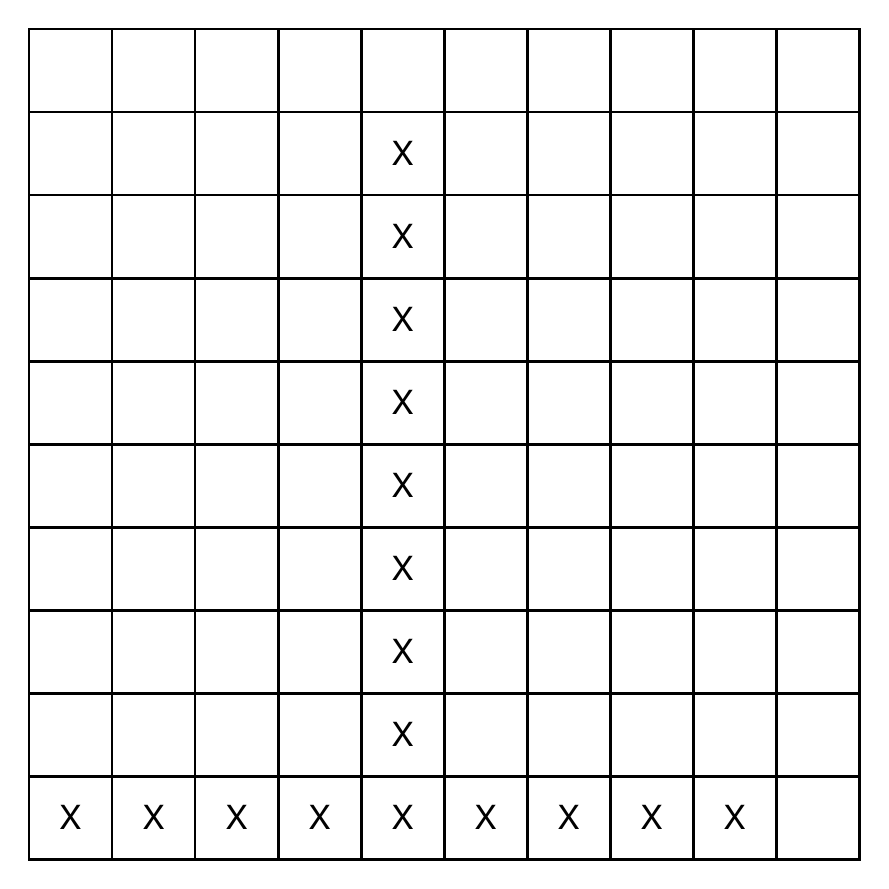
\begin{tikzpicture}[inner sep=0pt,scale=1]
\node (n0) [minimum height=30.0pt, minimum width=30.0pt,at={(270pt,-150pt)}, fill=white, draw, line width=1.0pt,align=center,text width=11.634765625,font=\fontfamily{phv}\fontsize{12}{13}\selectfont, shape=rectangle] {};
\node (n1) [minimum height=30.0pt, minimum width=30.0pt,at={(300pt,-150pt)}, fill=white, draw, line width=1.0pt,align=center,text width=11.634765625,font=\fontfamily{phv}\fontsize{12}{13}\selectfont, shape=rectangle] {};
\node (n2) [minimum height=30.0pt, minimum width=30.0pt,at={(330pt,-150pt)}, fill=white, draw, line width=1.0pt,align=center,text width=11.634765625,font=\fontfamily{phv}\fontsize{12}{13}\selectfont, shape=rectangle] {};
\node (n3) [minimum height=30.0pt, minimum width=30.0pt,at={(360pt,-150pt)}, fill=white, draw, line width=1.0pt,align=center,text width=11.634765625,font=\fontfamily{phv}\fontsize{12}{13}\selectfont, shape=rectangle] {};
\node (n4) [minimum height=30.0pt, minimum width=30.0pt,at={(390pt,-150pt)}, fill=white, draw, line width=1.0pt,align=center,text width=11.634765625,font=\fontfamily{phv}\fontsize{12}{13}\selectfont, shape=rectangle] {};
\node (n5) [minimum height=30.0pt, minimum width=30.0pt,at={(420pt,-150pt)}, fill=white, draw, line width=1.0pt,align=center,text width=11.634765625,font=\fontfamily{phv}\fontsize{12}{13}\selectfont, shape=rectangle] {};
\node (n6) [minimum height=30.0pt, minimum width=30.0pt,at={(450pt,-150pt)}, fill=white, draw, line width=1.0pt,align=center,text width=11.634765625,font=\fontfamily{phv}\fontsize{12}{13}\selectfont, shape=rectangle] {};
\node (n7) [minimum height=30.0pt, minimum width=30.0pt,at={(480pt,-150pt)}, fill=white, draw, line width=1.0pt,align=center,text width=11.634765625,font=\fontfamily{phv}\fontsize{12}{13}\selectfont, shape=rectangle] {};
\node (n8) [minimum height=30.0pt, minimum width=30.0pt,at={(510pt,-150pt)}, fill=white, draw, line width=1.0pt,align=center,text width=11.634765625,font=\fontfamily{phv}\fontsize{12}{13}\selectfont, shape=rectangle] {};
\node (n9) [minimum height=30.0pt, minimum width=30.0pt,at={(540pt,-150pt)}, fill=white, draw, line width=1.0pt,align=center,text width=19.26953125,font=\fontfamily{phv}\fontsize{12}{13}\selectfont, shape=rectangle] {};
\node (n10) [minimum height=30.0pt, minimum width=30.0pt,at={(270pt,-180pt)}, fill=white, draw, line width=1.0pt,align=center,text width=19.26953125,font=\fontfamily{phv}\fontsize{12}{13}\selectfont, shape=rectangle] {};
\node (n11) [minimum height=30.0pt, minimum width=30.0pt,at={(300pt,-180pt)}, fill=white, draw, line width=1.0pt,align=center,text width=19.26953125,font=\fontfamily{phv}\fontsize{12}{13}\selectfont, shape=rectangle] {};
\node (n12) [minimum height=30.0pt, minimum width=30.0pt,at={(330pt,-180pt)}, fill=white, draw, line width=1.0pt,align=center,text width=19.26953125,font=\fontfamily{phv}\fontsize{12}{13}\selectfont, shape=rectangle] {};
\node (n13) [minimum height=30.0pt, minimum width=30.0pt,at={(360pt,-180pt)}, fill=white, draw, line width=1.0pt,align=center,text width=19.26953125,font=\fontfamily{phv}\fontsize{12}{13}\selectfont, shape=rectangle] {};
\node (n14) [minimum height=30.0pt, minimum width=30.0pt,at={(390pt,-180pt)}, fill=white, draw, line width=1.0pt,align=center,text width=19.26953125,font=\fontfamily{phv}\fontsize{12}{13}\selectfont, shape=rectangle] {X};
\node (n15) [minimum height=30.0pt, minimum width=30.0pt,at={(420pt,-180pt)}, fill=white, draw, line width=1.0pt,align=center,text width=19.26953125,font=\fontfamily{phv}\fontsize{12}{13}\selectfont, shape=rectangle] {};
\node (n16) [minimum height=30.0pt, minimum width=30.0pt,at={(450pt,-180pt)}, fill=white, draw, line width=1.0pt,align=center,text width=19.26953125,font=\fontfamily{phv}\fontsize{12}{13}\selectfont, shape=rectangle] {};
\node (n17) [minimum height=30.0pt, minimum width=30.0pt,at={(480pt,-180pt)}, fill=white, draw, line width=1.0pt,align=center,text width=19.26953125,font=\fontfamily{phv}\fontsize{12}{13}\selectfont, shape=rectangle] {};
\node (n18) [minimum height=30.0pt, minimum width=30.0pt,at={(510pt,-180pt)}, fill=white, draw, line width=1.0pt,align=center,text width=19.26953125,font=\fontfamily{phv}\fontsize{12}{13}\selectfont, shape=rectangle] {};
\node (n19) [minimum height=30.0pt, minimum width=30.0pt,at={(540pt,-180pt)}, fill=white, draw, line width=1.0pt,align=center,text width=19.26953125,font=\fontfamily{phv}\fontsize{12}{13}\selectfont, shape=rectangle] {};
\node (n20) [minimum height=30.0pt, minimum width=30.0pt,at={(270pt,-210pt)}, fill=white, draw, line width=1.0pt,align=center,text width=19.26953125,font=\fontfamily{phv}\fontsize{12}{13}\selectfont, shape=rectangle] {};
\node (n21) [minimum height=30.0pt, minimum width=30.0pt,at={(300pt,-210pt)}, fill=white, draw, line width=1.0pt,align=center,text width=19.26953125,font=\fontfamily{phv}\fontsize{12}{13}\selectfont, shape=rectangle] {};
\node (n22) [minimum height=30.0pt, minimum width=30.0pt,at={(330pt,-210pt)}, fill=white, draw, line width=1.0pt,align=center,text width=19.26953125,font=\fontfamily{phv}\fontsize{12}{13}\selectfont, shape=rectangle] {};
\node (n23) [minimum height=30.0pt, minimum width=30.0pt,at={(360pt,-210pt)}, fill=white, draw, line width=1.0pt,align=center,text width=19.26953125,font=\fontfamily{phv}\fontsize{12}{13}\selectfont, shape=rectangle] {};
\node (n24) [minimum height=30.0pt, minimum width=30.0pt,at={(390pt,-210pt)}, fill=white, draw, line width=1.0pt,align=center,text width=19.26953125,font=\fontfamily{phv}\fontsize{12}{13}\selectfont, shape=rectangle] {X};
\node (n25) [minimum height=30.0pt, minimum width=30.0pt,at={(420pt,-210pt)}, fill=white, draw, line width=1.0pt,align=center,text width=19.26953125,font=\fontfamily{phv}\fontsize{12}{13}\selectfont, shape=rectangle] {};
\node (n26) [minimum height=30.0pt, minimum width=30.0pt,at={(450pt,-210pt)}, fill=white, draw, line width=1.0pt,align=center,text width=19.26953125,font=\fontfamily{phv}\fontsize{12}{13}\selectfont, shape=rectangle] {};
\node (n27) [minimum height=30.0pt, minimum width=30.0pt,at={(480pt,-210pt)}, fill=white, draw, line width=1.0pt,align=center,text width=19.26953125,font=\fontfamily{phv}\fontsize{12}{13}\selectfont, shape=rectangle] {};
\node (n28) [minimum height=30.0pt, minimum width=30.0pt,at={(510pt,-210pt)}, fill=white, draw, line width=1.0pt,align=center,text width=19.26953125,font=\fontfamily{phv}\fontsize{12}{13}\selectfont, shape=rectangle] {};
\node (n29) [minimum height=30.0pt, minimum width=30.0pt,at={(540pt,-210pt)}, fill=white, draw, line width=1.0pt,align=center,text width=19.26953125,font=\fontfamily{phv}\fontsize{12}{13}\selectfont, shape=rectangle] {};
\node (n30) [minimum height=30.0pt, minimum width=30.0pt,at={(270pt,-240pt)}, fill=white, draw, line width=1.0pt,align=center,text width=19.26953125,font=\fontfamily{phv}\fontsize{12}{13}\selectfont, shape=rectangle] {};
\node (n31) [minimum height=30.0pt, minimum width=30.0pt,at={(300pt,-240pt)}, fill=white, draw, line width=1.0pt,align=center,text width=19.26953125,font=\fontfamily{phv}\fontsize{12}{13}\selectfont, shape=rectangle] {};
\node (n32) [minimum height=30.0pt, minimum width=30.0pt,at={(330pt,-240pt)}, fill=white, draw, line width=1.0pt,align=center,text width=19.26953125,font=\fontfamily{phv}\fontsize{12}{13}\selectfont, shape=rectangle] {};
\node (n33) [minimum height=30.0pt, minimum width=30.0pt,at={(360pt,-240pt)}, fill=white, draw, line width=1.0pt,align=center,text width=19.26953125,font=\fontfamily{phv}\fontsize{12}{13}\selectfont, shape=rectangle] {};
\node (n34) [minimum height=30.0pt, minimum width=30.0pt,at={(390pt,-240pt)}, fill=white, draw, line width=1.0pt,align=center,text width=19.26953125,font=\fontfamily{phv}\fontsize{12}{13}\selectfont, shape=rectangle] {X};
\node (n35) [minimum height=30.0pt, minimum width=30.0pt,at={(420pt,-240pt)}, fill=white, draw, line width=1.0pt,align=center,text width=19.26953125,font=\fontfamily{phv}\fontsize{12}{13}\selectfont, shape=rectangle] {};
\node (n36) [minimum height=30.0pt, minimum width=30.0pt,at={(450pt,-240pt)}, fill=white, draw, line width=1.0pt,align=center,text width=19.26953125,font=\fontfamily{phv}\fontsize{12}{13}\selectfont, shape=rectangle] {};
\node (n37) [minimum height=30.0pt, minimum width=30.0pt,at={(480pt,-240pt)}, fill=white, draw, line width=1.0pt,align=center,text width=19.26953125,font=\fontfamily{phv}\fontsize{12}{13}\selectfont, shape=rectangle] {};
\node (n38) [minimum height=30.0pt, minimum width=30.0pt,at={(510pt,-240pt)}, fill=white, draw, line width=1.0pt,align=center,text width=19.26953125,font=\fontfamily{phv}\fontsize{12}{13}\selectfont, shape=rectangle] {};
\node (n39) [minimum height=30.0pt, minimum width=30.0pt,at={(540pt,-240pt)}, fill=white, draw, line width=1.0pt,align=center,text width=19.26953125,font=\fontfamily{phv}\fontsize{12}{13}\selectfont, shape=rectangle] {};
\node (n40) [minimum height=30.0pt, minimum width=30.0pt,at={(270pt,-270pt)}, fill=white, draw, line width=1.0pt,align=center,text width=19.26953125,font=\fontfamily{phv}\fontsize{12}{13}\selectfont, shape=rectangle] {};
\node (n41) [minimum height=30.0pt, minimum width=30.0pt,at={(300pt,-270pt)}, fill=white, draw, line width=1.0pt,align=center,text width=19.26953125,font=\fontfamily{phv}\fontsize{12}{13}\selectfont, shape=rectangle] {};
\node (n42) [minimum height=30.0pt, minimum width=30.0pt,at={(330pt,-270pt)}, fill=white, draw, line width=1.0pt,align=center,text width=19.26953125,font=\fontfamily{phv}\fontsize{12}{13}\selectfont, shape=rectangle] {};
\node (n43) [minimum height=30.0pt, minimum width=30.0pt,at={(360pt,-270pt)}, fill=white, draw, line width=1.0pt,align=center,text width=19.26953125,font=\fontfamily{phv}\fontsize{12}{13}\selectfont, shape=rectangle] {};
\node (n44) [minimum height=30.0pt, minimum width=30.0pt,at={(390pt,-270pt)}, fill=white, draw, line width=1.0pt,align=center,text width=19.26953125,font=\fontfamily{phv}\fontsize{12}{13}\selectfont, shape=rectangle] {X};
\node (n45) [minimum height=30.0pt, minimum width=30.0pt,at={(420pt,-270pt)}, fill=white, draw, line width=1.0pt,align=center,text width=19.26953125,font=\fontfamily{phv}\fontsize{12}{13}\selectfont, shape=rectangle] {};
\node (n46) [minimum height=30.0pt, minimum width=30.0pt,at={(450pt,-270pt)}, fill=white, draw, line width=1.0pt,align=center,text width=19.26953125,font=\fontfamily{phv}\fontsize{12}{13}\selectfont, shape=rectangle] {};
\node (n47) [minimum height=30.0pt, minimum width=30.0pt,at={(480pt,-270pt)}, fill=white, draw, line width=1.0pt,align=center,text width=19.26953125,font=\fontfamily{phv}\fontsize{12}{13}\selectfont, shape=rectangle] {};
\node (n48) [minimum height=30.0pt, minimum width=30.0pt,at={(510pt,-270pt)}, fill=white, draw, line width=1.0pt,align=center,text width=19.26953125,font=\fontfamily{phv}\fontsize{12}{13}\selectfont, shape=rectangle] {};
\node (n49) [minimum height=30.0pt, minimum width=30.0pt,at={(540pt,-270pt)}, fill=white, draw, line width=1.0pt,align=center,text width=19.26953125,font=\fontfamily{phv}\fontsize{12}{13}\selectfont, shape=rectangle] {};
\node (n50) [minimum height=30.0pt, minimum width=30.0pt,at={(270pt,-300pt)}, fill=white, draw, line width=1.0pt,align=center,text width=19.26953125,font=\fontfamily{phv}\fontsize{12}{13}\selectfont, shape=rectangle] {};
\node (n51) [minimum height=30.0pt, minimum width=30.0pt,at={(300pt,-300pt)}, fill=white, draw, line width=1.0pt,align=center,text width=19.26953125,font=\fontfamily{phv}\fontsize{12}{13}\selectfont, shape=rectangle] {};
\node (n52) [minimum height=30.0pt, minimum width=30.0pt,at={(330pt,-300pt)}, fill=white, draw, line width=1.0pt,align=center,text width=19.26953125,font=\fontfamily{phv}\fontsize{12}{13}\selectfont, shape=rectangle] {};
\node (n53) [minimum height=30.0pt, minimum width=30.0pt,at={(360pt,-300pt)}, fill=white, draw, line width=1.0pt,align=center,text width=19.26953125,font=\fontfamily{phv}\fontsize{12}{13}\selectfont, shape=rectangle] {};
\node (n54) [minimum height=30.0pt, minimum width=30.0pt,at={(390pt,-300pt)}, fill=white, draw, line width=1.0pt,align=center,text width=19.26953125,font=\fontfamily{phv}\fontsize{12}{13}\selectfont, shape=rectangle] {X};
\node (n55) [minimum height=30.0pt, minimum width=30.0pt,at={(420pt,-300pt)}, fill=white, draw, line width=1.0pt,align=center,text width=19.26953125,font=\fontfamily{phv}\fontsize{12}{13}\selectfont, shape=rectangle] {};
\node (n56) [minimum height=30.0pt, minimum width=30.0pt,at={(450pt,-300pt)}, fill=white, draw, line width=1.0pt,align=center,text width=19.26953125,font=\fontfamily{phv}\fontsize{12}{13}\selectfont, shape=rectangle] {};
\node (n57) [minimum height=30.0pt, minimum width=30.0pt,at={(480pt,-300pt)}, fill=white, draw, line width=1.0pt,align=center,text width=19.26953125,font=\fontfamily{phv}\fontsize{12}{13}\selectfont, shape=rectangle] {};
\node (n58) [minimum height=30.0pt, minimum width=30.0pt,at={(510pt,-300pt)}, fill=white, draw, line width=1.0pt,align=center,text width=19.26953125,font=\fontfamily{phv}\fontsize{12}{13}\selectfont, shape=rectangle] {};
\node (n59) [minimum height=30.0pt, minimum width=30.0pt,at={(540pt,-300pt)}, fill=white, draw, line width=1.0pt,align=center,text width=19.26953125,font=\fontfamily{phv}\fontsize{12}{13}\selectfont, shape=rectangle] {};
\node (n60) [minimum height=30.0pt, minimum width=30.0pt,at={(270pt,-330pt)}, fill=white, draw, line width=1.0pt,align=center,text width=19.26953125,font=\fontfamily{phv}\fontsize{12}{13}\selectfont, shape=rectangle] {};
\node (n61) [minimum height=30.0pt, minimum width=30.0pt,at={(300pt,-330pt)}, fill=white, draw, line width=1.0pt,align=center,text width=19.26953125,font=\fontfamily{phv}\fontsize{12}{13}\selectfont, shape=rectangle] {};
\node (n62) [minimum height=30.0pt, minimum width=30.0pt,at={(330pt,-330pt)}, fill=white, draw, line width=1.0pt,align=center,text width=19.26953125,font=\fontfamily{phv}\fontsize{12}{13}\selectfont, shape=rectangle] {};
\node (n63) [minimum height=30.0pt, minimum width=30.0pt,at={(360pt,-330pt)}, fill=white, draw, line width=1.0pt,align=center,text width=19.26953125,font=\fontfamily{phv}\fontsize{12}{13}\selectfont, shape=rectangle] {};
\node (n64) [minimum height=30.0pt, minimum width=30.0pt,at={(390pt,-330pt)}, fill=white, draw, line width=1.0pt,align=center,text width=19.26953125,font=\fontfamily{phv}\fontsize{12}{13}\selectfont, shape=rectangle] {X};
\node (n65) [minimum height=30.0pt, minimum width=30.0pt,at={(420pt,-330pt)}, fill=white, draw, line width=1.0pt,align=center,text width=19.26953125,font=\fontfamily{phv}\fontsize{12}{13}\selectfont, shape=rectangle] {};
\node (n66) [minimum height=30.0pt, minimum width=30.0pt,at={(450pt,-330pt)}, fill=white, draw, line width=1.0pt,align=center,text width=19.26953125,font=\fontfamily{phv}\fontsize{12}{13}\selectfont, shape=rectangle] {};
\node (n67) [minimum height=30.0pt, minimum width=30.0pt,at={(480pt,-330pt)}, fill=white, draw, line width=1.0pt,align=center,text width=19.26953125,font=\fontfamily{phv}\fontsize{12}{13}\selectfont, shape=rectangle] {};
\node (n68) [minimum height=30.0pt, minimum width=30.0pt,at={(510pt,-330pt)}, fill=white, draw, line width=1.0pt,align=center,text width=19.26953125,font=\fontfamily{phv}\fontsize{12}{13}\selectfont, shape=rectangle] {};
\node (n69) [minimum height=30.0pt, minimum width=30.0pt,at={(540pt,-330pt)}, fill=white, draw, line width=1.0pt,align=center,text width=19.26953125,font=\fontfamily{phv}\fontsize{12}{13}\selectfont, shape=rectangle] {};
\node (n70) [minimum height=30.0pt, minimum width=30.0pt,at={(270pt,-360pt)}, fill=white, draw, line width=1.0pt,align=center,text width=19.26953125,font=\fontfamily{phv}\fontsize{12}{13}\selectfont, shape=rectangle] {};
\node (n71) [minimum height=30.0pt, minimum width=30.0pt,at={(300pt,-360pt)}, fill=white, draw, line width=1.0pt,align=center,text width=19.26953125,font=\fontfamily{phv}\fontsize{12}{13}\selectfont, shape=rectangle] {};
\node (n72) [minimum height=30.0pt, minimum width=30.0pt,at={(330pt,-360pt)}, fill=white, draw, line width=1.0pt,align=center,text width=19.26953125,font=\fontfamily{phv}\fontsize{12}{13}\selectfont, shape=rectangle] {};
\node (n73) [minimum height=30.0pt, minimum width=30.0pt,at={(360pt,-360pt)}, fill=white, draw, line width=1.0pt,align=center,text width=19.26953125,font=\fontfamily{phv}\fontsize{12}{13}\selectfont, shape=rectangle] {};
\node (n74) [minimum height=30.0pt, minimum width=30.0pt,at={(390pt,-360pt)}, fill=white, draw, line width=1.0pt,align=center,text width=19.26953125,font=\fontfamily{phv}\fontsize{12}{13}\selectfont, shape=rectangle] {X};
\node (n75) [minimum height=30.0pt, minimum width=30.0pt,at={(420pt,-360pt)}, fill=white, draw, line width=1.0pt,align=center,text width=19.26953125,font=\fontfamily{phv}\fontsize{12}{13}\selectfont, shape=rectangle] {};
\node (n76) [minimum height=30.0pt, minimum width=30.0pt,at={(450pt,-360pt)}, fill=white, draw, line width=1.0pt,align=center,text width=19.26953125,font=\fontfamily{phv}\fontsize{12}{13}\selectfont, shape=rectangle] {};
\node (n77) [minimum height=30.0pt, minimum width=30.0pt,at={(480pt,-360pt)}, fill=white, draw, line width=1.0pt,align=center,text width=19.26953125,font=\fontfamily{phv}\fontsize{12}{13}\selectfont, shape=rectangle] {};
\node (n78) [minimum height=30.0pt, minimum width=30.0pt,at={(510pt,-360pt)}, fill=white, draw, line width=1.0pt,align=center,text width=19.26953125,font=\fontfamily{phv}\fontsize{12}{13}\selectfont, shape=rectangle] {};
\node (n79) [minimum height=30.0pt, minimum width=30.0pt,at={(540pt,-360pt)}, fill=white, draw, line width=1.0pt,align=center,text width=19.26953125,font=\fontfamily{phv}\fontsize{12}{13}\selectfont, shape=rectangle] {};
\node (n80) [minimum height=30.0pt, minimum width=30.0pt,at={(270pt,-390pt)}, fill=white, draw, line width=1.0pt,align=center,text width=19.26953125,font=\fontfamily{phv}\fontsize{12}{13}\selectfont, shape=rectangle] {};
\node (n81) [minimum height=30.0pt, minimum width=30.0pt,at={(300pt,-390pt)}, fill=white, draw, line width=1.0pt,align=center,text width=19.26953125,font=\fontfamily{phv}\fontsize{12}{13}\selectfont, shape=rectangle] {};
\node (n82) [minimum height=30.0pt, minimum width=30.0pt,at={(330pt,-390pt)}, fill=white, draw, line width=1.0pt,align=center,text width=19.26953125,font=\fontfamily{phv}\fontsize{12}{13}\selectfont, shape=rectangle] {};
\node (n83) [minimum height=30.0pt, minimum width=30.0pt,at={(360pt,-390pt)}, fill=white, draw, line width=1.0pt,align=center,text width=19.26953125,font=\fontfamily{phv}\fontsize{12}{13}\selectfont, shape=rectangle] {};
\node (n84) [minimum height=30.0pt, minimum width=30.0pt,at={(390pt,-390pt)}, fill=white, draw, line width=1.0pt,align=center,text width=19.26953125,font=\fontfamily{phv}\fontsize{12}{13}\selectfont, shape=rectangle] {X};
\node (n85) [minimum height=30.0pt, minimum width=30.0pt,at={(420pt,-390pt)}, fill=white, draw, line width=1.0pt,align=center,text width=19.26953125,font=\fontfamily{phv}\fontsize{12}{13}\selectfont, shape=rectangle] {};
\node (n86) [minimum height=30.0pt, minimum width=30.0pt,at={(450pt,-390pt)}, fill=white, draw, line width=1.0pt,align=center,text width=19.26953125,font=\fontfamily{phv}\fontsize{12}{13}\selectfont, shape=rectangle] {};
\node (n87) [minimum height=30.0pt, minimum width=30.0pt,at={(480pt,-390pt)}, fill=white, draw, line width=1.0pt,align=center,text width=19.26953125,font=\fontfamily{phv}\fontsize{12}{13}\selectfont, shape=rectangle] {};
\node (n88) [minimum height=30.0pt, minimum width=30.0pt,at={(510pt,-390pt)}, fill=white, draw, line width=1.0pt,align=center,text width=19.26953125,font=\fontfamily{phv}\fontsize{12}{13}\selectfont, shape=rectangle] {};
\node (n89) [minimum height=30.0pt, minimum width=30.0pt,at={(540pt,-390pt)}, fill=white, draw, line width=1.0pt,align=center,text width=19.26953125,font=\fontfamily{phv}\fontsize{12}{13}\selectfont, shape=rectangle] {};
\node (n90) [minimum height=30.0pt, minimum width=30.0pt,at={(270pt,-420pt)}, fill=white, draw, line width=1.0pt,align=center,text width=19.26953125,font=\fontfamily{phv}\fontsize{12}{13}\selectfont, shape=rectangle] {X};
\node (n91) [minimum height=30.0pt, minimum width=30.0pt,at={(300pt,-420pt)}, fill=white, draw, line width=1.0pt,align=center,text width=19.26953125,font=\fontfamily{phv}\fontsize{12}{13}\selectfont, shape=rectangle] {X};
\node (n92) [minimum height=30.0pt, minimum width=30.0pt,at={(330pt,-420pt)}, fill=white, draw, line width=1.0pt,align=center,text width=19.26953125,font=\fontfamily{phv}\fontsize{12}{13}\selectfont, shape=rectangle] {X};
\node (n93) [minimum height=30.0pt, minimum width=30.0pt,at={(360pt,-420pt)}, fill=white, draw, line width=1.0pt,align=center,text width=19.26953125,font=\fontfamily{phv}\fontsize{12}{13}\selectfont, shape=rectangle] {X};
\node (n94) [minimum height=30.0pt, minimum width=30.0pt,at={(390pt,-420pt)}, fill=white, draw, line width=1.0pt,align=center,text width=19.26953125,font=\fontfamily{phv}\fontsize{12}{13}\selectfont, shape=rectangle] {X};
\node (n95) [minimum height=30.0pt, minimum width=30.0pt,at={(420pt,-420pt)}, fill=white, draw, line width=1.0pt,align=center,text width=19.26953125,font=\fontfamily{phv}\fontsize{12}{13}\selectfont, shape=rectangle] {X};
\node (n96) [minimum height=30.0pt, minimum width=30.0pt,at={(450pt,-420pt)}, fill=white, draw, line width=1.0pt,align=center,text width=19.26953125,font=\fontfamily{phv}\fontsize{12}{13}\selectfont, shape=rectangle] {X};
\node (n97) [minimum height=30.0pt, minimum width=30.0pt,at={(480pt,-420pt)}, fill=white, draw, line width=1.0pt,align=center,text width=19.26953125,font=\fontfamily{phv}\fontsize{12}{13}\selectfont, shape=rectangle] {X};
\node (n98) [minimum height=30.0pt, minimum width=30.0pt,at={(510pt,-420pt)}, fill=white, draw, line width=1.0pt,align=center,text width=19.26953125,font=\fontfamily{phv}\fontsize{12}{13}\selectfont, shape=rectangle] {X};
\node (n99) [minimum height=30.0pt, minimum width=30.0pt,at={(540pt,-420pt)}, fill=white, draw, line width=1.0pt,align=center,text width=26.904296875,font=\fontfamily{phv}\fontsize{12}{13}\selectfont, shape=rectangle] {};
\end{tikzpicture}
\caption{Here, the score for the player $X$ is 4}
\end{center}
\end{figure}


%\begin{description}
%	\item[empty] ist der Seitenstil, bei dem Kopf- und Fusszeile vollständig 	leer bleiben.\marginpar[\textit{Randnotiz links}]
%	{\textit{Randnotiz rechts}}
%    \item[plain] ist der Seitenstil, bei dem keinerlei Kolumnentitel verwendet wird.
%    \item[headings] ist der Seitenstil für automatische Kolumnentitel.
%    \item[myheadings] ist der Seitenstil für manuelle Kolumnentitel.
%\end{description}



%$\mathsf{({m}^{3}/s)}$
%-------------------------------
%\begin{figure}
%	\setcapindent{-1em}
%    \fbox{\parbox{.95\linewidth}{
%    	\centering\KOMAScript}}
%	\caption{Beispiel mit teilweise hängendem Einzug ab der zweiten Zeile}
%\end{figure}

%Guten Morgen\footnote{irgend ein text\label{refnote}}\multiplefootnoteseparator\footnote{es geht noch weiter}Blabla\footref{refnote}
\end{document}
